\subsection{Wellen am Doppelspalt} \label{subsec:doppelspalt}

Wenn nun ein Bündel mit jeweils räumlich und zeitlich kohärenten Wellen (Vergleiche Abbildung \ref{fig:brechung} und \referenz{subsec:interferenz}) auf ein Hindernis mit 2 schmalen Spalten trifft, bilden sich dahinter auf einem dort aufgestellten Schirm zeitlich stabile Interferenzen.

Die Interferenzen werden durch die Überlagerung von Wellen verursacht, in diesem Fall von den zwei Wellen, die, gemäß dem Huygen'schen Prinzip, von den Spalten ausgehen. Ein beliebiger Punkt hinter dem Spalt hat einen unterschiedlichen Abstand zu den beiden Schlitzen, das heißt es kann sein, dass sich an diesem Punkt sowohl ein Wellenberg von der einen Welle als auch ein Wellenberg der anderen Welle treffen und zu einem noch höheren Maximum addieren. Allerdings ist auch das umgekehrte Extrem und jedes Dazwischen möglich.

\begin{figure}[!h]
	\center
	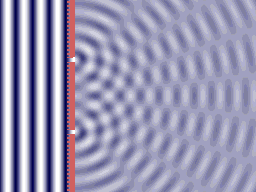
\includegraphics[width=0.7\textwidth]{doppelspalt}
	\caption{Kohärente Welle am Doppelspalt, man kann sie sich als Wasserwellen vorstellen.}
	\label{fig:doppelspaltwasser}
\end{figure}

Diese Ausbreitung (man betrachte Grafik \ref{fig:doppelspaltwasser} \footnote{Animiertes .gif von: \url{https://www.itp.uni-hannover.de/~zawischa/ITP/beugg.html}}) der zwei Wellen hinter den Spalten ist mit dem Huygens'schen Prinzip (\referenz{subsec:ausbreitung}) zu erklären: Angenommen, in jedem Spalt gäbe es nur ein schwingendes Teilchen. Dieses wird von der Wellenfront erfasst und ist selber Auslöser einer zirkularen Welle. Da dieser Oszillator an dieser Stelle der einzige ist, gibt es keine gerade Wellenfront als Einhüllende, sondern einzig die Zirkularwelle des angeregten Oszillators.

Natürlich gibt es immer mehr als nur ein Teilchen im Spalt, aber wenn der Spalt einigermaßen klein ist, ist die resultierende Welle immer noch annähernd kreisförmig, mit Toleranzen, die bei der Mathematisierung zu vernachlässigen sind.


\subsubsection{Mathematisierung}

Der Versuch ist mit Laserlicht durchführbar, welches monochromatisch (eine einzige Wellenlänge) und kohärent ist. Das Licht wird durch einen schmalen Doppelspalt mit dem Spaltabstand $d \leq 2mm$ hinter dem sich im Abstand $a$ ein Schirm befindet. 
	
Auf dem Schirm ist das Interferenzmuster zu beobachten. In der Mitte ist ein heller Streifen, links und rechts davon, symmetrisch, sind weniger intensive Lichtpunkte. Alle diese hellen Punkte werden Maxima genannt, da in diesen Punkten konstruktive Interferenz herrscht (\referenz{subsec:interferenz}). An den Minimalstellen herrschen destruktive Interferenzen. Der Gangunterschied ergibt sich hier durch den unterschiedlichen Abstand der Punkte auf dem Schirm zu dem beiden Schlitzen.

Eine Zeichnung\footnote{„Double-slit schematic“ von Peter Suppenhuhn, svg version by Trutz Behn, modified by Till Blaha - Eigenes Werk. Lizenziert unter Gemeinfrei über Wikimedia Commons - \url{https://commons.wikimedia.org/wiki/File:Double-slit_schematic.svg}}:

\begin{figure}[h!]
		\centering
		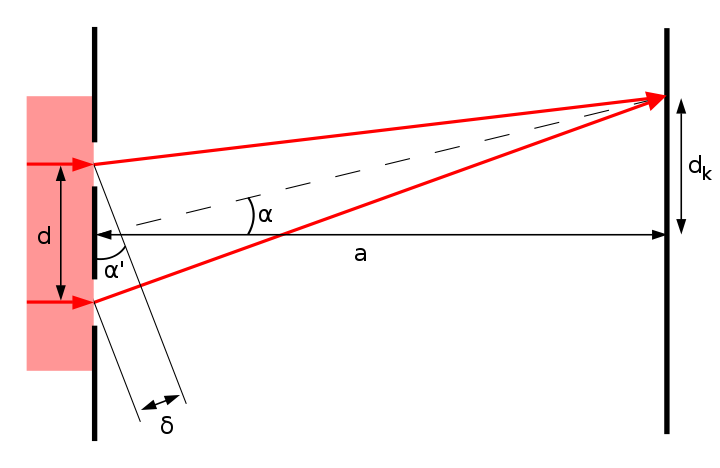
\includegraphics[width=0.8\textwidth]{doppelspaltzeichnung}
		\caption{Zeichnung zur Herleitung}
\end{figure}

Der helle Punkt in der Mitte ist das 0. Maximum, welches sich durch den exakt gleichen Abstand von \emph{beiden} Spalten ergibt. $k$ in der Gleichung \ref{eq:kon_interferenz} auf Seite \pageref{eq:kon_interferenz}.
	
Die Winkel $\alpha$ und $\alpha '$ sind gleich und werden im Folgen schlicht als $\alpha$ bezeichnet. Für $\alpha$ ergeben sich aus den trigonomischen Winkelfunktionen im rechtwinkligen Dreieck 2 Gleichungen: $sin{\alpha}=\frac{\delta}{d}$ und $tan{\alpha}=\frac{d_k}{a}$. Da $a>>d_k$ ist $\alpha<10 \degree$ und die Kleinwinkelnäherung $sin{\alpha} \approx \tan{\alpha}$ kann verwendet werden.

Der Gangunterschied $\delta$ muss der Bedingung für konstruktive Interferenz $\delta = k \cdot \lambda$ genügen (Siehe Gleichung \ref{eq:kon_interferenz} auf Seite \pageref{eq:kon_interferenz}). Daraus Ergibt sich:
	
\begin{align}
\begin{split}
	\sin{\alpha} &= \tan{\alpha} \\
	\frac{\delta}{d} &= \frac{d_k}{a} \\
	\frac{k \cdot \lambda}{d} &= \frac{d_k}{a} \quad \text{wobei} \ k \in 1,2,3... \\
	\lambda &= \frac{d_{k} \cdot d}{a \cdot k} \quad \text{wobei} \ k \in 1,2,3...
\end{split}
\end{align}
	
\noindent Für $k$ muss die Ordnung des betrachteten Maxima eingesetzt werden.
		

\subsubsection{Ohne Kleinwinkelnäherung}

Um die Wellenlänge präziser bestimmen zu können, kann der Spaltabstand verringert werden. Dann ist der Abstand zwischen den Maxima größer und man kann, relativ gesehen, den Abstand genauer bestimmen. Wenn man aber den Spaltabstand verringert, wird die Intensität des Lichtes kleiner, sodass man die Maxima kaum mehr erkennen kann. Dabei hilft man sich, indem man mehr als 2 Spalte verwendet, ein Gitter mit ca. 1000 Spalten und einem Spaltabstand in der Größenordnung von $\frac{1}{600}mm$.

Das Hinzufügen der Schlitze ändert allerdings nichts an den mathematischen Grundlagen des Versuchs.
	
Allerdings geht mit dem größeren Abstand der Punkte auf dem Schirm die Gültigkeit der Kleinwinkelnäherung verloren. Allerdings kann die Größe des Winkels $\alpha$ über $\arctan{\frac{d_k}{a}}$ berechnet werden und in die Gleichung $\sin{\alpha} = \frac{\delta}{d}$ eingesetzt werden:
	
\begin{align}
\begin{split}
		\frac{\delta}{d} &= \sin{\alpha} \\
		\delta &= \sin{(\arctan{\frac{d_k}{a}})} \cdot d \\
		\lambda \cdot k &= \sin{(\arctan{\frac{d_k}{a}})} \cdot d   \quad \text{wobei} \ k \in 1,2,3... \\
		\lambda &= \frac{\sin{(\arctan{\frac{d_k}{a}})} \cdot d}{k} \quad \text{wobei} \ k \in 1,2,3...
\end{split}
\end{align}


\subsection{Lichtspektrum am Doppelspalt}

Wenn ein Lichtspektrum (z.B. weißes Licht von einer Glühbirne) auf einen Doppelspalt oder ein Gitter trifft, welches weder monochromatisch noch kohärent ist, dann tritt ein ähnliches Phänomen wie bei monochromatischem Licht auf, das sich dahingehend unterscheidet, dass die unterschiedlichen Wellenlängen im Spektrum ihren eigenen, von der Wellenlänge abhängigen, Abstand $d_k$ haben. Dadurch wird das Lichtspektrum von violett bis rot aufgefächert (\glqq Dispersion\grqq ).

\begin{Aufgabe}
Wird violettes Licht in einer Dispersion, vom Mittelpunkt des Schirmes aus gesehen, außen oder innen im Spektrum liegen?
\end{Aufgabe}


\subsection{Interferenz an dünnen Schichten}	\label{subsec:duenneschicht}

Wenn Licht an sehr dünnen Schichten, die einen Teil des Lichtes durchlassen und dabei brechen, aber auch einen Teil reflektieren, kann es zur Interferenz bei den reflektierten Strahlen kommen. Häufig werden Seifenblasen oder Glimmerplättchen als Beispiel genannt, das Prinzip ist jedoch das gleiche. Für eine Beobachtung mit Spektrallicht folgt, dass in der Reflexion eine Wellenlänge, also eine Farbe, \glqq aus dem Spektrum gezogen wird\grqq{} und das reflektierte Licht diese nun nicht mehr enthält.


\subsection{Glimmerplättchen}

Ein Glimmerplättchen ist eine doppelreflektierende Schicht, sodass sich folgendes Bild für einen Lichtstrahl ergibt:

\begin{figure}[h!]
	\centering
	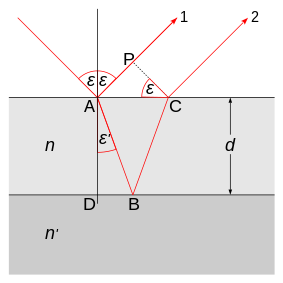
\includegraphics[width=0.6\textwidth]{duenneschicht}
	\caption{Der selbe Lichtstrahl wird zweimal reflektiert.}
\end{figure}

\begin{comment}
% Cue: wrong, needs improvement
Bei beiden Reflexionen ereignet sich ein Phasensprung von $\pi$ (Siehe: \referenz{subsec:Reflexion}), sodass sich für die Schichtdicke, in Abhängigkeit der auszulöschenden Wellenlänge, folgendes ergibt:
\end{comment}

Für die Schichtdicke $d$ ergibt sich, wenn man die Kleinwinkelnäherung anwendet, also $\overline{AB} =  \overline{BC} = d$, ergibt sich für die Schichtdicke in Abhängigkeit der auszulöschenden Wellenlänge:

\begin{align}
\begin{split}
	d = \frac{\lambda}{4} + k \cdot \lambda \quad wobei \ k \in 1,2,3 ...
\end{split}
\end{align}


\subsection{Optische Vergütung}











